\chapter{Evaluation} % (fold)
\label{cha:evaluation}

Für die Erprobung des Q-Learning-Algorithmus wurden zwei Linienfolger und eine Teststrecke konzipiert und aufgebaut. Der Kurs (siehe Abbildung \ref{fig:kurs}) besteht aus verschiedenen Geraden- und Kurvenstücken von variablem Schwierigkeitsgrad.

\begin{figure}[!htb]
	\centering
	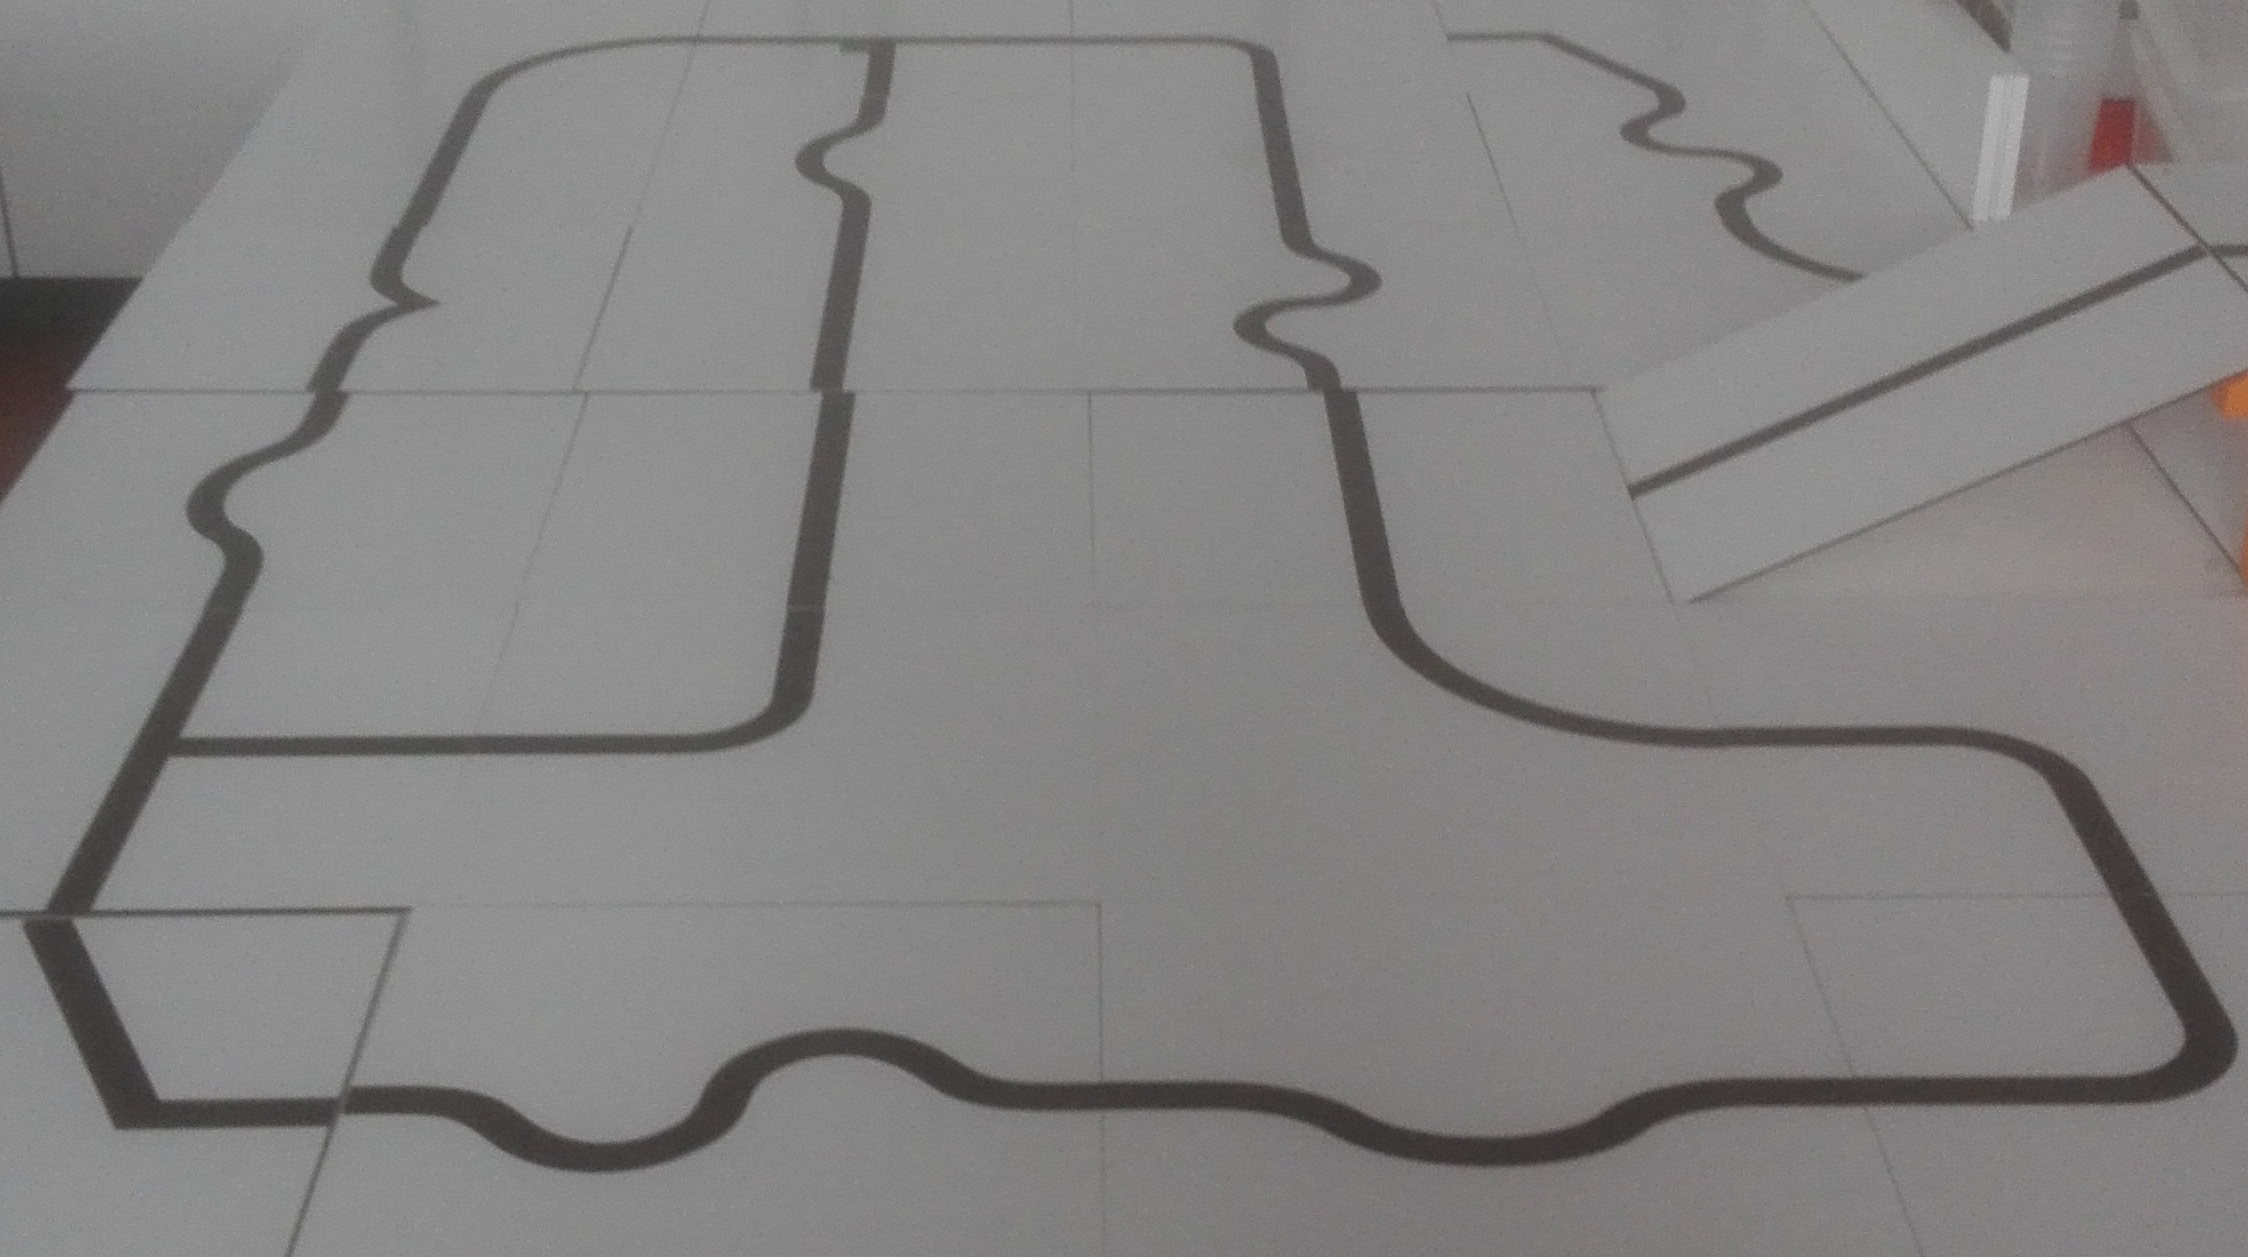
\includegraphics[width=8cm]{kurs.png}
	\caption{Kurs}
	\label{fig:kurs}
\end{figure}

Die beiden Linienfolger unterscheiden sich in der Anzahl und der Anordnung der Farbsensoren. Der erste Linienfolger $L_0$ verfügt über drei Farbsensoren (siehe Abbildung \ref{fig:linienfolger-drei-sensoren}), die nebeneinander angeordnet sind. Die schwarze Linie besitzt dieselbe Breite wie der Lichtkegel eines Farbsensors. Sommit ist der Linienfolger optimal Positioniert falls nur der mittlere Sensor Schwarz und die beiden außenliegenden Sensoren Weiß erkennen. Im Gegensatz zum ersten Linienfolger besitzt der zweite Linienfolger $L_1$ zwei Farbsensoren, die angewinkelt angeordnet sind (siehe Abbildung \ref{fig:linienfolger-zwei-sensoren}). Im optimalen Fall liegt die Linie genau in den sich überschneidenden Lichtkegeln der zwei Sensoren.

\begin{figure}[H]
    \centering
    \begin{minipage}{0.45\textwidth}
        \centering
        \includegraphics[width=0.9\textwidth]{linienfolger-drei-sensoren.png}
        \caption{$L_0$}
        \label{fig:linienfolger-drei-sensoren}
    \end{minipage}\hfill
    \begin{minipage}{0.45\textwidth}
        \centering
        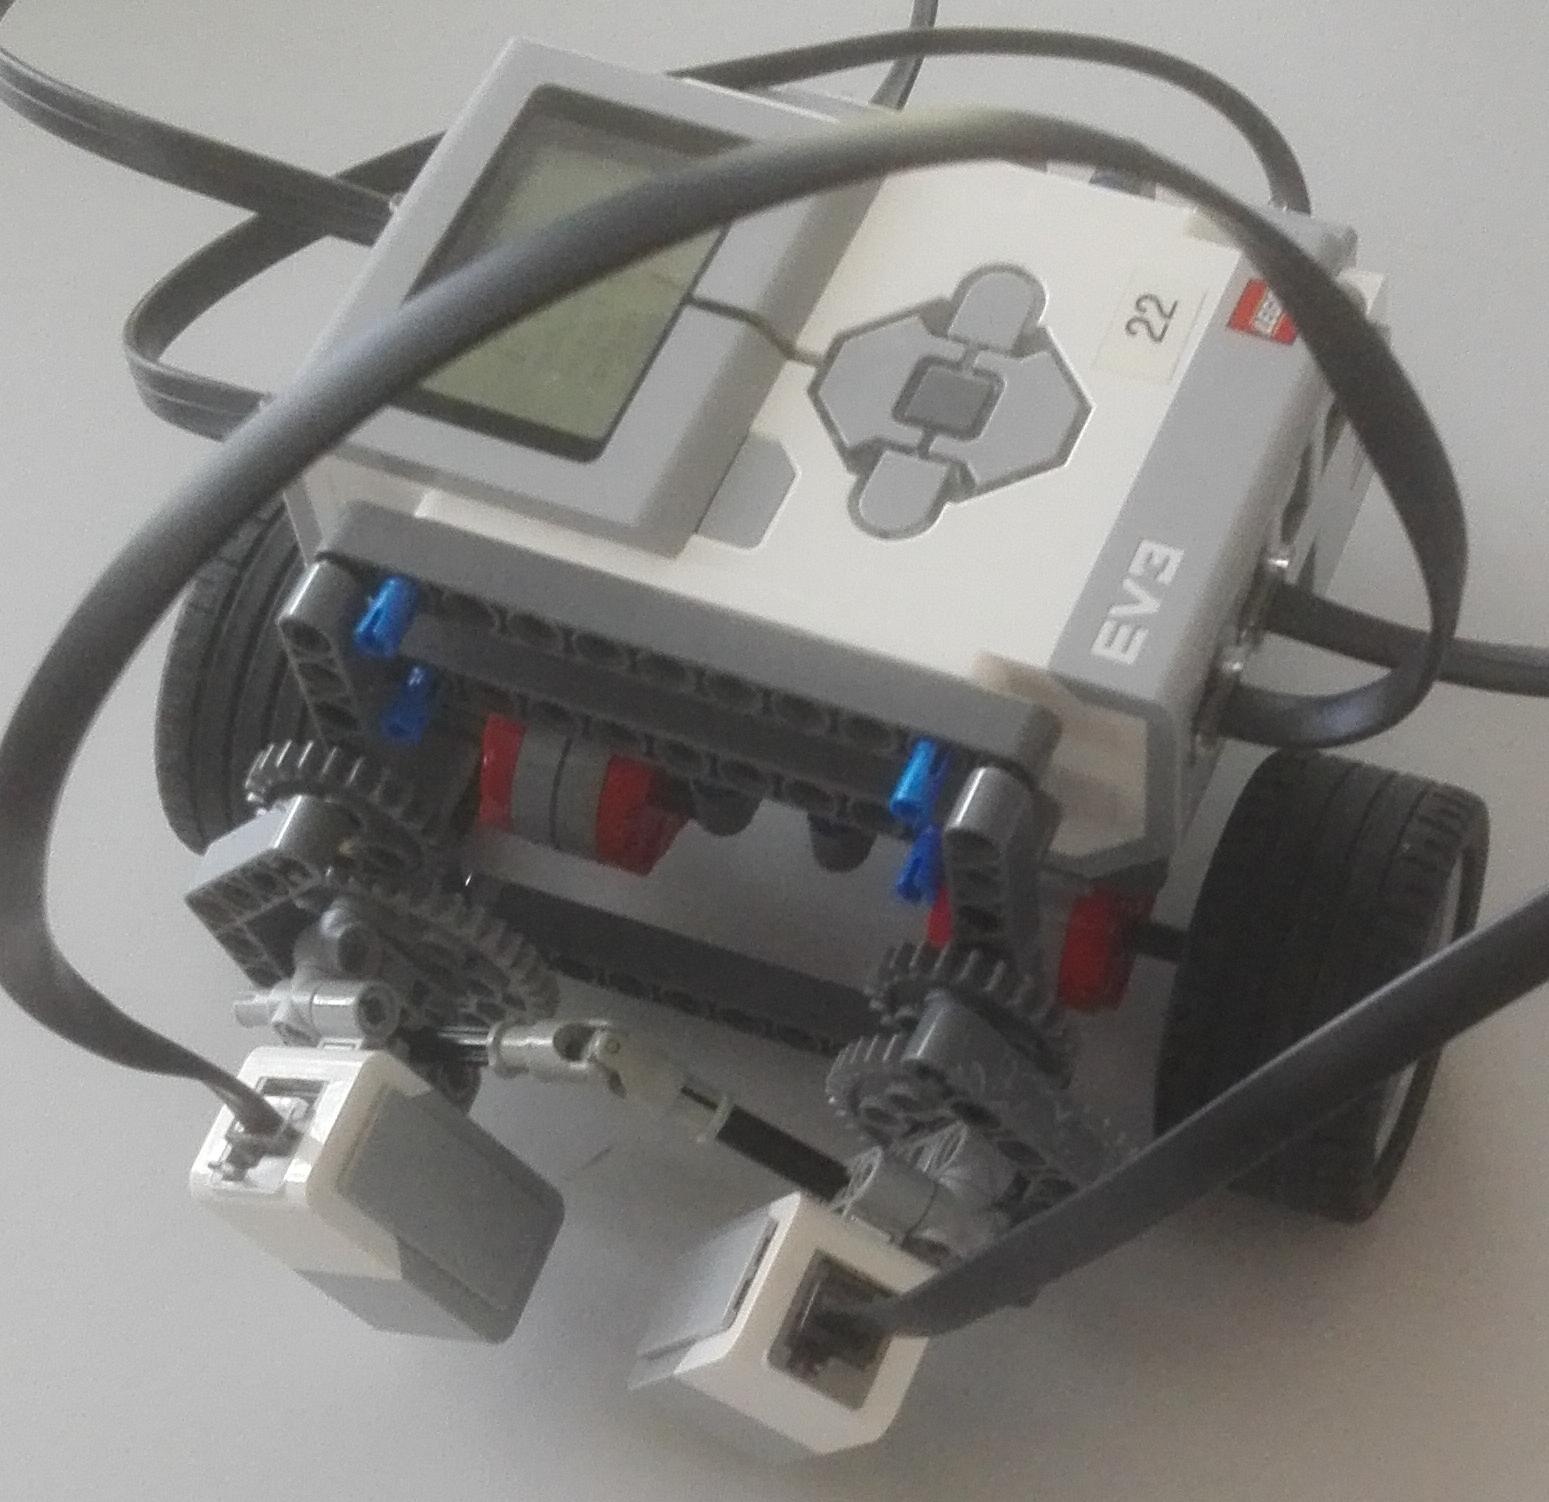
\includegraphics[width=0.9\textwidth]{linienfolger-zwei-sensoren.png}
        \caption{$L_1$}
        \label{fig:linienfolger-zwei-sensoren}
    \end{minipage}
\end{figure}

Die Sensoranordnungen der Linienfolger führt zu zwei unterschiedlichen Zustandsräumen. Die Zustände beider Linienfolger sind in den Tabellen \ref{tab:zustaende_drei_sensoren} und \ref{tab:zustaende_zwei_sensoren} angegeben.

\begin{table}[H]
  \caption{Zustandstabelle für $L_0$}
  \label{tab:zustaende_drei_sensoren}
  \renewcommand{\arraystretch}{1.2}
  \centering
  \sffamily
  \begin{footnotesize}
    \begin{tabular}{l l l}
    \toprule
    \textbf{Zustand} & \textbf{Beschreibung} & \textbf{Belohnung}\\
    \midrule
    $s_0$	&	Alle Sensoren erkennen Weiß.	&	0\\ % 000
    $s_1$	&	Der rechte Sensor erkennt Schwarz.	&	0\\ % 001
    $s_2$	&	Der mittlere Sensor erkennt Schwarz.	&	1\\ % 010
    $s_3$	&	Der mittlere und rechte Sensor erkennt Schwarz.	&	0\\ % 011
    $s_4$	&	Der linke Sensor erkennt Schwarz.	&	0\\ % 100
    $s_5$	&	Der linke und rechte Sensor erkennt Schwarz.	&	0\\ % 101
    $s_6$	&	Der linke und mittlere Sensor erkennt Schwarz.	&	0\\ % 110
    $s_7$	&	Alle Sensoren erkennen Schwarz.	&	0\\ % 111
    \bottomrule
    \end{tabular}
  \end{footnotesize}
  \rmfamily
\end{table}

\begin{table}[!htbp]
  \caption{Zustandstabelle für $L_1$}
  \label{tab:zustaende_zwei_sensoren}
  \renewcommand{\arraystretch}{1.2}
  \centering
  \sffamily
  \begin{footnotesize}
    \begin{tabular}{l l l}
    \toprule
    \textbf{Zustand} & \textbf{Beschreibung} & \textbf{Belohnung}\\
    \midrule
    $s_0$	&	Beide Sensoren erkennen Weiß.	&	0\\
    $s_1$	&	Der rechte Sensor erkennt Schwarz.	&	0\\
    $s_2$	&	Der linke Sensor erkennt Schwarz.	&	0\\
    $s_3$	&	Beide Sensoren erkennen Schwarz.	&	1\\
    \bottomrule
    \end{tabular}
  \end{footnotesize}
  \rmfamily
\end{table}

Zur Erreichung eines anderen Zustandes können beide Linienfolger folgende Aktionen (siehe Tabelle \ref{tab:aktionen}) ausführen. Beide Linienfolger benutzten die selben Motorgeschwindigkeiten und Ruhezeiten um die Vergleichbarkeit bei der Aktionsausführung zu garantieren. Beide Linienfolger nutzen für das Q-Learning die gleichen Parameter (siehe Tabelle \ref{tab:q-parameter}), um die Vergleichbarkeit der Ergebnisse zu gewährleisten.

\begin{table}[H]
  \caption{Aktionen}
  \label{tab:aktionen}
  \renewcommand{\arraystretch}{1.2}
  \centering
  \sffamily
  \begin{footnotesize}
    \begin{tabular}{l l}
    \toprule
    \textbf{Aktion} & \textbf{Beschreibung}\\
    \midrule
    $a_0$	&	Linkskurve\\
    $a_1$	&	Ge­ra­de­aus­fahrt\\
    $a_2$	&	Rechtskurve\\
    \bottomrule
    \end{tabular}
  \end{footnotesize}
  \rmfamily
\end{table}
\quad
\begin{table}[H]
  \caption{Q-Learning-Parameter}
  \label{tab:q-parameter}
  \renewcommand{\arraystretch}{1.2}
  \centering
  \sffamily
  \begin{footnotesize}
    \begin{tabular}{l l}
    \toprule
    \textbf{Parameter} & \textbf{Wert}\\
    \midrule
    $\alpha$	&	$0.9$\\
    $\gamma$	&	$0.2$\\
    $\epsilon$	&	$0.1$\\
    \bottomrule
    \end{tabular}
  \end{footnotesize}
  \rmfamily
\end{table}

Durch theoretische Überlegungen kommt man für beide Linienfolger auf optimale Aktionen, die für einen Zustand ausgeführt werden sollen. Während diese bei $L_1$ (siehe Abbildung \ref{fig:zwei_sensoren_optimale_strategie}) leicht herzuleiten sind, ist dies bei $L_0$ (siehe Abbildung \ref{fig:drei_sensoren_optimale_strategie}) durch den größeren Zustandsraum ungleich schwieriger.\footnote{Bei beiden Graphen wurden nicht alle möglichen sinvollen Aktionen angegeben.} Bei drei Sensoren liegen zwei Zustände $s_5$ und $s_7$ vor, die nicht optimal sind. $s_5$ kann nur angenommen werden, falls $L_0$ genau auf einer Linienlücke steht.

\begin{figure}[H]
    \centering
    \begin{minipage}{0.45\textwidth}
        \centering
        \begin{tikzpicture}[->,>=stealth',shorten >=1pt,auto,node distance=2cm,
                    thick,main node/.style={circle,draw,font=\sffamily\Large\bfseries}]

          \node[main node] (1) {$s_1$};
          \node[main node] (2) [below left of=1] {$s_0$};
          \node[main node] (3) [below right of=2] {$s_3$};
          \node[main node] (4) [below right of=1] {$s_2$};

          \path[every node/.style={font=\sffamily\small}]
            (1) edge node [left] {$a_0$} (3)
            (2) edge node [left] {$a_2$} (1)
                edge [bend below] node [top] {$a_1$} (4)
            (3) edge [loop below] node {$a_1$} (3)
            (4) edge node [left] {$a_2$} (3);
        \end{tikzpicture}
        \caption{Optimale Strategie bei zwei Sensoren}
        \label{fig:zwei_sensoren_optimale_strategie}
    \end{minipage}\hfill
    \begin{minipage}{0.45\textwidth}
        \centering
        \begin{tikzpicture}[->,>=stealth',shorten >=1pt,auto,node distance=2cm,
                    thick,main node/.style={circle,draw,font=\sffamily\Large\bfseries}]

          \node[main node] (1) {$s_2$};
          \node[main node] (2) [below left of=1] {$s_1$};
          \node[main node] (3) [below right of=1] {$s_3$};
          \node[main node] (4) [below left of=2] {$s_0$};
          \node[main node] (5) [below right of=3] {$s_4$};
          \node[main node] (6) [below right of=4] {$s_7$};
          \node[main node] (7) [below left of=5] {$s_5$};
          \node[main node] (8) [below right of=6] {$s_6$};


          \path[every node/.style={font=\sffamily\small}]
            (1) edge [loop above] node {$a_1$} (1)
            (2) edge node [above] {$a_2$} (3)
                edge [loop left] node {$a_2$} (2)
            (3) edge node [right] {$a_2$} (1)
            (4) edge node [left] {$a_2$} (2)
                edge [bend above] node [above] {$a_0$} (5)
            (5) edge [bend left] node {$a_0$} (8)
                edge [bend right] node [right] {$a_0$} (1)
            (6) edge node [left] {$a_0$} (8)
                edge [bend left] node [left] {$a_2$} (3)
            (7) edge node [left] {$a_0$} (5)
                edge [bend left] node [left] {$a_2$} (2)
            (8) edge [bend right] node [left below] {$a_0$} (1);
        \end{tikzpicture}
        \caption{Optimale Strategie bei drei Sensoren} 
        \label{fig:drei_sensoren_optimale_strategie}
    \end{minipage}
\end{figure}

Bei beiden Linienfolgern wurden die optimalen Aktionen für jeden Zustand alle 200 Lernschritte archiviert (siehe Tabelle \ref{tab:q-values-three-sensors} für $L_0$ und \ref{tab:q-values-two-sensors} für $L_1$). Ein Vergleich mit den theoretisch optimalen Werten zeigt eine Abweichung. Des Weitern fluktuieren die Aktionen auch nach 2000 Lernschritten für beide Linenfolger noch beträchtlich.

\begin{table}[h]
  \caption{Q-Werte für zwei Sensoren}
  \label{tab:q-values-two-sensors}
  \renewcommand{\arraystretch}{1.2}
  \centering
  \sffamily
  \begin{footnotesize}
    \begin{tabular}{l l l l l l l l l}
    \toprule
    \textbf{Schritte} & \textbf{$s_0$} & \textbf{$s_1$} & \textbf{$s_2$} & \textbf{$s_3$}\\
    \midrule
    200     &       $a_2$   &       $a_1$   &       $a_1$   &       $a_0$\\
    400  &       $a_0$   &       $a_0$   &       $a_0$   &       $a_1$\\
    600  &       $a_0$   &       $a_0$   &       $a_2$       &       $a_1$\\
    800  &       $a_0$   &       $a_2$   &       $a_1$   &       $a_1$\\
    1000 &       $a_1$   &       $a_2$   &       $a_0$   &       $a_2$\\
    1200 &       $a_1$   &  $a_1$    &       $a_1$   &       $a_0$\\
    1400 &       $a_0$   &       $a_1$   &       $a_0$   &       $a_0$\\
    1600 &       $a_2$   &       $a_0$   &       $a_0$   &       $a_2$\\
    1800 &  $a_2$    &       $a_2$   &       $a_1$   &       $a_2$\\
    2000 &       $a_2$   &       $a_2$   &       $a_0$   &       $a_0$\\
    \bottomrule
    \end{tabular}
  \end{footnotesize}
  \rmfamily
\end{table}

\begin{table}[h]
  \caption{Q-Werte für drei Sensoren}
  \label{tab:q-values-three-sensors}
  \renewcommand{\arraystretch}{1.2}
  \centering
  \sffamily
  \begin{footnotesize}
    \begin{tabular}{l l l l l l l l l}
    \toprule
    \textbf{Schritte} & \textbf{$s_0$} & \textbf{$s_1$} & \textbf{$s_2$} & \textbf{$s_3$} & \textbf{$s_4$} & \textbf{$s_5$} & \textbf{$s_6$} & \textbf{$s_7$}\\
    \midrule
    200     &       $a_0$   &       $a_1$   &       $a_2$   &       $a_0$   &       $a_0$   &       $a_2$   &       $a_0$   &       $a_0$\\
    400  &       $a_0$   &       $a_0$   &       $a_1$   &  $a_0$    &       $a_1$   &       $a_2$   &       $a_0$   &       $a_0$\\
    600  &       $a_1$   &       $a_2$   &       $a_2$   &       $a_0$   &       $a_1$   &       $a_2$   &       $a_0$   &  $a_2$\\
    800   &       $a_0$   &       $a_2$   &       $a_2$   &       $a_1$   &       $a_1$   &       $a_2$   &       $a_0$   &       $a_2$\\
    1000 &       $a_2$   &       $a_0$   &       $a_2$       &       $a_1$   &       $a_1$   &       $a_1$   &       $a_2$   &       $a_2$\\
    1200 &       $a_2$   &       $a_0$   &       $a_2$   &       $a_2$   &       $a_2$   &       $a_1$   &  $a_2$    &       $a_1$\\
    1400 &       $a_2$   &       $a_2$   &       $a_0$   &       $a_2$   &       $a_0$   &       $a_0$   &       $a_2$   &       $a_0$\\
    1600 &       $a_1$   &       $a_2$       &       $a_0$   &       $a_2$   &       $a_0$   &       $a_0$   &       $a_2$   &       $a_0$\\
    1800 &       $a_1$   &       $a_2$   &       $a_2$   &       $a_2$   &       $a_0$   &  $a_0$    &       $a_2$   &       $a_0$\\
    2000 &       $a_1$   &       $a_2$   &       $a_0$   &       $a_2$   &       $a_1$   &       $a_0$   &       $a_2$   &       $a_0$\\
    \bottomrule
    \end{tabular}
  \end{footnotesize}
  \rmfamily
\end{table}

Der Einsatz von drei Sensoren in $L_0$ führt zu neuen Schwierigkeiten, da für manche Zustände die optimale Lösung von der auftretenden Situation abhänig ist und sommit eine einmal gelerente Lösung zu einem späteren Zeitpunkt zu einer faschen Lösung führen kann.\par
Bei $L_1$ ist die gewinkelte Anordnung der Sensoren ein Problem, da die Lichtkegel der Sensoren sich nicht hundertprozentig überschneiden. Die beiden Lichtkegel überschneiden sich nur in den Außenbereichen. Dies läst sich aufgrund der vorgegebenen Legobauteile nicht vermeiden. Dies führt zu einer fehlerhaften Erkennung von $s_3$. Des Weiteren können die Sensoren aufgrund der Bauweise nicht star befestigt werden und schwanken sommit im Bereich der Lichtkegel. Dies führt zu Messungenauigkeiten. Bei drei Sensoren kann der Linienfolger zwischen den Zuständen $s_1$ und $s_4$ wechseln, ohne vom Fleck zu kommen. Dies kann durch Herabsetzung der Ruhezeiten oder der Motorgeschwindigkeit behoben werden.\par
Im Allgemeinen ist die optimale Kombination aus Ruhezeiten und Motorgeschwindigkeit von der Sensoranzahl und -anordnung abhängig. Diese ist bei beiden Linienfolgern noch nicht optimal. 

% chapter evaluation (end)